\documentclass[12pt]{article}

\usepackage{pgfplots}
\pgfplotsset{compat=1.18} % Or adjust depending on your TeX distribution
\usepackage[utf8]{inputenc}	% Para caracteres en español
\usepackage{amsmath,amsthm,amsfonts,amssymb,amscd}
\usepackage{multirow,booktabs}
\usepackage[table]{xcolor}
\usepackage{fullpage}
\usepackage{lastpage}
\usepackage{newtxtext}
\usepackage{newtxmath}
\usepackage{enumitem}
\usepackage{fancyhdr}
\usepackage{mathrsfs}
\usepackage{wrapfig}
\usepackage{setspace}
\usepackage{calc}
\usepackage{multicol}
\usepackage{cancel}
\usepackage[retainorgcmds]{IEEEtrantools}
\usepackage[margin=3cm]{geometry}
\usepackage{amsmath}
\newlength{\tabcont}
\setlength{\parindent}{0.0in}
\setlength{\parskip}{0.05in}
\usepackage{empheq}
\usepackage{framed}
\usepackage[most]{tcolorbox}
\usepackage{xcolor}
\colorlet{shadecolor}{orange!15}
\parindent 0in
\parskip 12pt
\geometry{margin=1in, headsep=0.25in}
\theoremstyle{definition}
\newtheorem{defn}{Definition}
\newtheorem{reg}{Rule}
\newtheorem{exer}{Exercise}
\newtheorem{note}{Note}
\newtheorem{theorem}{Theorem}
\setcounter{section}{0}
\usepackage{chngcntr}

\counterwithin*{equation}{section}
\counterwithin*{equation}{subsection}

\begin{document}

\section{Taylor}

Let $f \in C^n[a, b]$ and assume $f^{(n+1)}$ exists in $(a, b)$. Then 
for any $c, x \in [a, b]$ there is some $\zeta$ between $c$ and $x$ s.t. 

\begin{equation}
f(x) = \sum_{k=0}^{n} \frac{f^{(k)}(c)(x-c)^k}{k!} + E_n(x)
\end{equation}

where 

\begin{equation*}
    E_n(x) = \frac{f^{(n+1)}(\zeta)(x-c)^{n+1}}{(n+1)!}
\end{equation*}

Equation $(1)$ is called the Taylor expansion of $f$ around $c$. 

\begin{shaded}
    \textbf{Observation.} The famous \textit{mean value theorem} is simply the
    case $n = 0$ of Taylor's expansion: if $f \in C[a, b]$ and $f'$ exists on
    $(a, b)$, then for $x, c \in [a, b]$

    \begin{equation*}
        f(x) = f(c) + f'(\zeta)(x-c)
    \end{equation*}

    where $\zeta$ is between $c$ and $x$. Take $x=b, c = a$ and the theorem
    appears:

    \begin{equation*}
        f(b) - f(a) = f'(\zeta)(b-a)
    \end{equation*}
\end{shaded}

We typically extend the Taylor approximation of $f$ around a point $r$, where
$r = x + h$ is an approximation some value of interest $x$. This is useful
because said approximation gives 

\begin{equation*}
    f(r) = f(x+h) = f(x) + f'(x)h + \frac{ f^{''}(x) }{2}h^2 + \ldots + 
    \frac{ f^{(n)}(x) }{n!}h^n + E_n(h)
\end{equation*}

In other words, this strategy allows us to extend $f(r)$ in terms of $x$ and
$h$, the approximation and its error. Usually, $r, h$ are unknown but $h$ can be
bounded.

\pagebreak

\section{Alg. de Horner: Polynomial evaluation} 

Consider 

\begin{equation*}
    p(x) = \sum_{i=0}^n a_ix^i
\end{equation*}

We wish to compute $p(k)$ for a given $k \in \mathbb{R}$ minimizing the number
of operations. Directly computing $a_0 + a_1k_1 + \ldots$ leads to $n$ sums. The
$i$th term requires computing $k^i$, which means $i$ product operations, for a
totall of $\sum_{i=1}^n i = \frac{n(n+1)}{2}$ products.  The total number of
operations is then 

\begin{equation*}
    \Theta = n + n(n+1) / 2
\end{equation*}

The associated complexity is $\mathcal{O}(n^2)$. 

Horner's method consists of re-writing $p(x)$ so that the number of products is
reduced. One writes 

\begin{equation*}
    p(x) = a_0 + x b_0
\end{equation*}

where $b_{n-1} = a_n$ and for $0 \leq i < n - 1$:

\begin{equation*}
    b_{i-1} = a_{i} + xb_{i}
\end{equation*}

\begin{shaded}
    \begin{example}
        \normalfont
        Let $p(x) = 3 + 5x -4x^2 + 0x^3 + 6x^4$, giving $n = 4$. Then 
        $b_{3} = 6$ and 

        \begin{align*}
            &b_2 = a_3 + xb_3 = 6x,  &b_1 = a_2 + xb_2 = -4 + x(6x),\\
            &b_0 = a_1 + xb_1 = 5 + x(-4+x(6x)) 
        \end{align*}

        This finally gives

        \begin{equation*}
            p(x) = 3 + xb_0 = 3+x(5 +
            x(-4+x(6x)))
        \end{equation*}
    \end{example}
\end{shaded}

Here, one must perform $n$ sums again but only $n$ products. Thus, there are
$\Theta = n + n = 2n$ operations, giving a complexity of $\mathcal{O}(n)$ (in
the operation space). See the algorithm below:

\begin{align*}
&\textbf{input } n; a_i, i = 0, \ldots, n; x \\ 
& b_{n-1} \leftarrow a_n \\ 
& \textbf{for } i = n - 2 \textbf{ to } i = 0 \\ 
&\qquad b_{i} = a_{i+1} + x * b_{i+1} \\ 
&\textbf{od}\\
&y \leftarrow a_0 + x*b_0 \\ 
&\textbf{return } y
\end{align*}

It is easy to see in this code that the $\textbf{for}$ loop performs $n-1$
iterations, in each of which a single sum and a single product are computed. The
$n$th sum and $n$th product are performed in the computation of $y$, the final
result. 

A more polished version includes the last computatoin (the one in the assignment
of $y$) within the loop and makes no use of indexes:


\begin{align*}
&\textbf{input } n; a_i, i = 0, \ldots, n; x \\ 
& b \leftarrow a_n \\ 
& \textbf{for } i = n - 2 \textbf{ to } i = -1 \\ 
&\qquad b = a_{i+1} + x * b \\ 
&\textbf{od}\\
&\textbf{return } b
\end{align*}
 
In Python,


\small
\begin{quote}


\begin{verbatim}
def horner(coefs, x):
  n = len(coefs)-1
  b = coefs[n]

  for i in reversed(range(-1, n-1)):
    b = coefs[i+1] + x*b

  return b

\end{verbatim}

\end{quote}
\normalsize


It is trivial to adapt the code so that it returns the coefficients $b_0,
\ldots, b_{n-1}$ and not the final result, if needed.

\pagebreak 

\section{Error}

Let $r, \overline{r}$ be two real numbers s.t. the latter is an approximation of
the first. We define the \textbf{error} of the approximation to be $r -
\hat{r}$, and 

\begin{align*}
    \Delta r = \left| r - \overline{r} \right|, \qquad \delta r = \frac{\Delta
    r}{\left| r \right| }
\end{align*}

With $r$ unknown the strategy is to work with a known bound of $r$.

\pagebreak 

\section{Non-linear equations}

The general problem is to find members of the set $\mathcal{R}_f$ of roots of $f
\in \mathbb{R} \to \mathbb{R}$. The numerical strategy is to iteratively
approximate some $r \in \mathcal{R}_f$ until some pre-established threshold in
the error of approximation is met. 

More formally, the numerical strategy produces a sequence $\left\{ x_k
\right\}_{k\in \mathbb{N}}
$ which satisfies 

\begin{itemize}
    \item $\lim_{k\to \infty} \left\{ x_k \right\} = r$  for some $r \in
        \mathcal{R}_f$ 
    \item Either $e(x_k) < e(x_{k-1})$ or, more strongly, $\lim_{k\to \infty}
        e(x_k) = 0$, where $e(x_k)$ is some appropriate measure of the error of
        approximation.
\end{itemize}

\subsection{Bisection}

A very simple procedure: if a root exists in $[a, b]$, it iteratively shrinks
$[a,b]$ in halves (keeping the halves which contain the root) until the interval
is of sufficiently small length or the root is found.

\begin{theorem}[Intermediate value]
    If $f$ is continuous in $[a, b]$ and $f(a)f(b) < 0$, then $\exists r \in
    \mathcal{R}_f$ s.t. $r \in [a, b]$.
\end{theorem}

Assume $f$ is continuous. A root exists in $[a, b]$ if $f(a)f(b) < 0$
(\textbf{Theorem 1}). If that is the case, the midpoint $(a+b) / 2$ is taken as
the approximation $x_0$. It is also trivial to observe that $x_0$ is \textit{at
most} at a distance of $(b-a) / 2$ from the real root, so $e_0 = |x_0 - r| \leq
(b-a) / 2$. 

If $f(x_0) = 0$ the procedure must end because a root was found. Otherwise,
sufficies to find which half of the interval contains a root computing
$f(a)f(c)$ and, if needed, $f(c)f(b)$.

The iterations may stop after reaching a maximum number of steps, when $|f(c)|$
is sufficiently close to zero, or when the error bound $|e_k| \leq (b_k - a_k) /
2$ (where $[a_k, b_k]$ is the interval of this iteration) is sufficiently small.

\begin{shaded}
    \textbf{(!)} The algorithm not always converges. Take $f(x) = 1 / x$. Clearly, it has no
    root. Yet setting $a = -1, b=1$ in the initial iteration falsely passes the
    test. (The problem obviously is that $f$ is not continuous in $[-1, 1]$.) If
    one sets
\end{shaded}

\pagebreak 

\begin{align*}
&\textbf{Input}: a, b, \delta, M, f\\  
&\textbf{Output}: \text{Tupla de la forma: } (r, \text{cota de error})\\
&f_a \leftarrow  f(a) \\ 
&f_b \leftarrow f(b) \\ 
&\qquad\\
&\textbf{if } f_a*f_b > 0 \\ 
&\qquad \textbf{return } ?\\ 
&\textbf{fi}\\
&\qquad\\
&\textbf{for } i = 1 \textbf{ to } i = M \textbf{ do } \\ 
&\qquad c \leftarrow a + (b-a) / 2 \\ 
&\qquad f_c \leftarrow f(c) \\ 
&\qquad \textbf{if } f_c = 0 \textbf{ then } \\ 
&\qquad\qquad \textbf{ return } (c, 0) \\ 
&\qquad\textbf{fi}\\
&\qquad \epsilon = \frac{b - a}{2}\\
&\qquad \textbf{if } \epsilon < \delta \textbf{ then } \\ 
& \qquad\qquad \textbf{break}\\
&\qquad\textbf{fi}\\
&\qquad \textbf{if } f_a*f_c < 0 \textbf{ then } \\ 
&\qquad \qquad b \leftarrow c \\ 
&\qquad\qquad f_b = f(b)\\
&\qquad\textbf{else } \\ 
&\qquad\qquad a \leftarrow c \\ 
&\qquad\qquad f_a = f(a)\\
&\qquad\textbf{fi} \\ 
&\textbf{od}\\
&\textbf{return } (c, \epsilon)
\end{align*}

\pagebreak 


\small
\begin{quote}

\begin{verbatim}
def bisection(f : callable, a : float, b : float, delta : float, M : int):

  s, e = f(a), f(b) # function values at (s)tart, (e)nd of interval

  if s*e > 0:
    raise ValueError("Interval [a, b] contains no root.")

  for i in range(M):

    c = a + (b-a)/2 
    m = f(c) # value of f at (m)idpoint

    if m == 0:
      return c, 0

    e = (b-a)/2
    if e < delta:
      return c, e

    if s*m < 0:
      b = c 
      e = f(b)
    else:
      a = c 
      s = f(a)
    
  return c, e

\end{verbatim}

\end{quote}
\normalsize

\pagebreak

\begin{theorem}
    If $\left\{ [a_i, b_i] \right\}_{i=0}^\infty $ are the intervals generated
    by the bisection method on iterations $i = 0, 1, \ldots$, then:

    \begin{enumerate}
        \item $\lim_{n\to
    \infty} a_n = \lim_{n \to \infty} b_n$ is a member of $\mathcal{R}_f$.
     \item If $c_n = \frac{1}{2}(a_n + b_n), r = \lim_{n \to \infty} c_n $, then 
         $|r - c_n| \leq \frac{1}{2^{n+1}}(b_0 - a_0)$
    \end{enumerate}

\end{theorem}


\small
\begin{quote}

\textbf{Proof.} \textbf{(1)} It is clear that $a_i \leq a_{i+1}$ and $b_i \geq b_{i+1}$,
since the interval on each iteration shrinks in one direction. 

$\therefore a_n, b_n$ are monotonous. 

But clearly $a_n$ is bounded by $b_0$ and $b_n$ is bounded by $a_0$. 

$\therefore $ $a_n, b_n$ are monotonous and bounded. 

$\therefore $ Their limits exist.

It is also clear that the interval shrinks to half its size on each iteration: 

\begin{equation}
    b_n - a_n = \frac{1}{2} (b_{n-1} - a_{n-1}), \qquad n \geq 1
\end{equation}

By recurrence on $(1)$,

\begin{equation}
    b_n - a_n = \frac{1}{2^n}(b_0 - a_0), \qquad n \geq 0
\end{equation}

Then 

\begin{equation}
   \lim_{n \to \infty} a_n - \lim_{n \to \infty} b_n = \lim_{n \to \infty} (a_n - b_n) 
    = \lim_{n \to \infty}  \frac{1}{2^n}(b_0 - a_0) = 0
\end{equation}

$\therefore ~ \lim_{n \to \infty} a_n = \lim_{n \to \infty} b_n$.


Since the limit of $a_n, b_n$ exists and $f$ is by assumption continuous, the
composition limit theorem applies and:

\begin{align}
    &\lim_{n \to \infty} \left( f(a_n) \cdot f(b_n) \right) \nonumber
\\
    =& \lim_{n \to \infty}    f(a_n) \cdot \lim_{n \to \infty} f(b_n) &\left\{ \text{Product of limits} \right\}  \nonumber \\ 
    =& f\left( \lim_{n \to \infty} a_n
\right) \cdot f\left( \lim_{n \to \infty} b_n \right)  &\left\{
\text{Composition limit theorem} \right\} \nonumber \\ 
    =& \left[ f(r) \right]^2 &\left\{ r = \lim_{n \to \infty} a_n \right\} 
\end{align}

The invariant of the algorithm is $f(a_n)f(b_n) < 0$. But due to the last
result,

\begin{equation*}
    \lim_{n \to \infty} f(a_n)f(b_n) \leq 0 \iff [f(r)]^2 \leq 0 \iff f(r) = 0
\end{equation*}

$\therefore r = \lim_{n \to \infty} a_n = \lim_{n \to \infty} b_n$ is a root.

\textbf{(2)} Follows directly from result $(2)$

\begin{align*}
    \left| r - c_n \right|  &= \left| r - \frac{1}{2}(b_n - a_n) \right| \\ 
                            &\leq
    \left| \frac{1}{2}(b_n - a_n) \right| \\ 
&=\left| \frac{1}{2^{n+1}}(b_0 - a_0) \right| &\left\{ \text{Result }(2)
\right\} 
\end{align*}



\end{quote}
\normalsize

\pagebreak 

\subsection{Newton's method}


Assume $r \in \mathcal{R}_f$ and $r = x + h$, with $x$ an approximation of $r$
and $h$ its error. Assume $f''$ exists and is continuous in some $I$ around $x$
s.t. $r \in I$. What we explained on Taylor expansions around a point gives:

\begin{equation*}
    0 = f(r) = f(x + h) = f(x) + f'(x)h + \mathcal{O}(h^2)
\end{equation*}

If $x$ is sufficiently close to $r$, $h$ is small and $h^2$ even smaller, so
that $\mathcal{O}(h^2)$ is unconsiderable:

\begin{equation*}
    0 \approx f(x) + hf'(x)
\end{equation*}

Therefore, 

\begin{equation}
    h \approx - \frac{f(x)}{f'(x)}
\end{equation}

From this follows that $r = x + h$ is approximated by 

\begin{equation*}
    r \approx x - \frac{f(x)}{f'(x)}
\end{equation*}

Since the approximation in $(5)$ truncated the terms of $\mathcal{O}(h^2)$
complexity, this new approximation is closer to $r$ than $x$ originally was. In
other words, $x - f(x) / f'(x)$ is a better approximation to $r$ than $x$
itself. 

Thus, if $x_0$ is an original approximation, we can define 

\begin{equation}
    x_{n+1} = x_n - \frac{f(x_n)}{f'(x_n)}
\end{equation}

to produce a sequence of approximations. This is the fundamental idea of
Newton's method.

\begin{align*}
&\textbf{Input: } x_0, M, \delta, \epsilon; \\ 
&v \leftarrow f(x_0) \\ 
&\textbf{if } |v| < \epsilon \textbf{ then return }  x_0 \textbf{ fi }\\ 
&\textbf{for } k = 1 \textbf{ to } k = M \textbf{ do } \\ 
&\qquad x_1 \leftarrow x_0 - \frac{v}{f'(x_0)} \\
&\qquad v \leftarrow f(x_1) \\ 
&\qquad \textbf{if } \left| x_1 - x_0 \right| < \delta \lor v < \epsilon
\textbf{ then } \\ 
&\qquad\qquad \textbf{return } x_1 \\ 
&\qquad\textbf{fi} \\ 
&\qquad x_0 \leftarrow x_1 \\ 
&\textbf{od} \\ 
&\textbf{return } x_0
\end{align*}

The predicate $\left| x_1 - x_0 \right| < \delta$ checks whether our algorithm
is adjusting $x$ in a negligible degree. If that is the case, we
should stop. 

\begin{theorem}
    If $f''$ continuous around $r \in \mathcal{R}_f$ and $f'(r) \neq 0$, then
    there is some $\delta > 0$ s.t. if $\left| r - x_0 \right| \leq \delta $,
    then: 

    \begin{itemize}
        \item $\left| r - x_n \right| \leq \delta $ for all $n \geq 1$. 
        \item $\left\{ x_n \right\} $ converges to $r$  
        \item The convergence is quadratic, i.e. there is a constant $c(\delta)$
            and a natural $N$ s.t. $\left| r - x_{n+1} \right| \leq c\left| r -
            x_n\right|^2  $ for all $n \geq N$.
    \end{itemize}

\end{theorem}



\small
\begin{quote}

\textbf{Proof.} Let $e_n = r - x_n$ be the error in the $n$th approximation. Assume $f''$ is
continuous and $f(r) = 0$, $f'(r) \neq 0$. Then 

\begin{align}
    e_{n+1} &= r-  x_{n+1}  \nonumber \\ 
&= r - \left( x_n - \frac{f(x_n)}{f'(x_n)} \right) \nonumber \\ 
&= r - x_n  + \frac{f(x_n)}{f'(x_n)}\nonumber \\
&=\frac{e_n f'(x_n) + f(x_n)}{f'(x_n)}
\end{align}

Thus, the error at any given iteration is a function of the error at the
previous iteration. Now consider the expansion of $f(r)$ as 

\begin{equation}
    f(r) = f(x_n - e_n) = f(x_n) + e_nf'(x_n) + \frac{e_n^2f''(\zeta_n)}{2}
\end{equation}

for $\zeta_n$ between $x_n$ and $r$. This equation gives 

\begin{equation}
    e_n f'(x_n) + f(x_n) = -\frac{1}{2} f''(\zeta_n)e_n^2
\end{equation}

The expression in $(5)$ is the numerator in $(3)$, whereby we obtain via
substitution: 

\begin{equation}
    e_{n+1} =  -\frac{1}{2}\frac{f''(\zeta_n)e^2_n}{f'(x_n)} 
\end{equation}

Equation $(6)$ ensures that the error scales quadratically. Now we wish to
bound the error expression in $(6)$. To bound $e_{n+1}$, we take
$\delta > 0$ to define a neighbourhood of length $\delta$ around $r$. For any
$x$ in this neighbourhood, $(6)$ reaches its maximum when the numerator is
maximized and the denominator is minimized:

\begin{equation*}
    c(\delta) = \frac{1}{2} \frac{ \max_{\left| x - r \right| \leq \delta }
    \left| f''(x) \right|  }{\min_{\left| x-r \right| \leq \delta \left| f'(x) \right|  }}
\end{equation*}

In other words, $c(\delta)$ is the maximum value which $e_{n+1}$ can take if
$\zeta_n, x_n$ are assumed to belong to the neighbourhood. Now we make two
assumptions: 

\begin{enumerate}
    \item $x_0$ belongs to the neighbourhood, i.e. $\left| x_0 - r \right| \leq
        \delta$ 
    \item $\delta$ is sufficiently small so that $\varrho := \delta c(\delta) < 1$.
\end{enumerate}

Note that, since $\zeta_0$ is between $x_0$ and $r$, assumption (1) ensures that
$\zeta_0$ is also in the neighbourhood, i.e. $\left| r - \zeta_0 \right| \leq
\delta$. Then we have:

\begin{equation*}
    \left| e_0 \right| = \frac{1}{2} \left| f''(\zeta_0) / f'(x_0) \right| \leq c(\delta)
\end{equation*}

Then:

\begin{align*}
    \left| x_1 - r \right|  
    &= \left| e_1 \right|  \\ 
    &= \left| e_0^2 \cdot \frac{1}{2} f''(\zeta_0) / f'(x_0)  \right|  \\ 
    &\leq |e_0^2| c(\delta) &\left\{ \frac{1}{2}f''(\zeta_0) / f'(x_0) \leq c(\delta) \right\}  \\ 
    &\leq |e_0| \delta c(\delta) &\left\{ \left| e_0 \right| \leq \delta
    \right\}  \\ 
    &=\left| e_0 \right| \varrho &\left\{ \varrho = \delta c(\delta) \right\} \\
    &< \left| e_0 \right|  &\left\{ \varrho < 1 \right\}  \\ 
    &\leq \delta
\end{align*}

$\therefore $ $\left| e_1 \right| < \left| e_0 \right| \leq \delta$, which means
the error decreases. This argument may be repeated inductively, giving:
 
\begin{align*}
    &\left| e_1 \right|  \leq \varrho \left| e_0 \right|  \\ 
    &\left| e_2 \right|  \leq \varrho \left| e_1 \right| \leq \varrho^2 \left| e_0 \right|   \\ 
    &\left| e_3 \right|  \leq \varrho \left| e_2 \right| \leq \varrho^3 \left| e_0 \right|   \\ 
    &\vdots
\end{align*}

In general, $\left| e_{n} \right| \leq \varrho^n \left| e_0 \right|
$. And since $0 \leq \varrho < 1$, we have $\varrho^n \to 0$ when $n \to \infty$,
entailing that $\left| e_n \right| \to 0$ when $n \to \infty$.
\end{quote}
\normalsize

\begin{theorem}
    If $f''$ is continuous in $\mathbb{R}$, and if $f$ is increasing, convex,
    and has a root, then said root is unique and Newton's method converges to it
    from any starting point.
\end{theorem}

\begin{shaded}
    Recall that $f$ is convex if $f''(x) > 0$ for all $x$. Graphically, it is
    convex if the line connecting two arbitrary points of $f$ lies above the
    curve of $f$ between those two points.
\end{shaded}


\subsection{Secant method}

In Netwon's method, 

\begin{equation*}
    x_{n+1} = x_n - \frac{f(x_n)}{f'(x_n)}
\end{equation*}

The function of interest is $f$. We cannot escape computing $f(x_n)$, but it
would be desirable to avoid the computation of $f'(x_n)$, which may potentially
be expensive. Since

\begin{equation*}
    f'(x) = \lim_{h \to x}  \frac{f(x) - f(h)}{x-h}
\end{equation*}

it is natural to suggest 

\begin{equation}
    f'(x_n) \approx \frac{f(x_n) - f(x_{n-1})}{x_n - x_{n-1}}
\end{equation}

Graphically, this means we are not using the line tangent to the point $(x_n,
f(x_n))$ but the line secant to the points $(x_n, f(x_n)$ and $(x_{n-1},
f(x_{n-1}))$. The point $x_{n+1}$ is then the value of $x$ where this secant
line has a root.

\subsection{Fixed point iteration}

The key observation is  this: if $r \in \mathcal{R}_f$, then $g(x) = x - kf(x)$
has $r$ as fixed point, for any $k \in \mathbb{R}$. Inversely, if $g$ has a
fixed point in $r$, then $r \in \mathcal{R}_f$. 

\begin{theorem}
    (1) Let $g \in C[a, b]$ and assume $g(x) \in [a, b]$ for all $x \in [a, b]$.
    Then there is a  fixed point of $g$ in $[a, b]$.

    (2) If, on top of previous conditions, $g$ is differentiable in $(a, b)$ and
    there is some $k < 1$ s.t. $\left| g'(x) \right| \leq k$ for all $x \in
    (a,b)$, then the fixed point referred in (1) is unique.
\end{theorem}

\begin{shaded}
    \begin{theorem}[Mean value theorem]
        Let $f : [a, b] \to \mathbb{R}$ continuous and differentiable on $(a,
        b)$ with $a < b$. Then there is some $c \in (a, b)$  s.t. 

        \begin{equation*}
            f'(c) = \frac{ f(b) - f(a) }{b - a}
        \end{equation*}
    \end{theorem}

    The interpretation is simple: consider the line secant to $f$ on $a, b$. The
    theorem ensures that there is some point $c$ s.t. the line tangent to $c$ is
    parallelt to said secant (equal slopes).
\end{shaded}

\small
\begin{quote}

\textbf{Proof.} (1) If $a$ or $b$ are fixed points the proof is done so assume
otherwise. Since $g(x) \in [a, b]$,  we have $g(a) > a$ and $g(b) < b$.


Take $\varphi(x) = g(x) - x$, which is continuous and defined in $[a,
b]$. Then 

\begin{equation*}
    \varphi(a) = g(a) - a > 0, \qquad \varphi(b) = g(b) - b < 0
\end{equation*}

Then $\varphi(a)\varphi(b) < 0$. Then, by the intermediate value theorem,
$\varphi$ has a root in $(a, b)$. In otherwords, there is at least one $p$ s.t. 

\begin{equation*}
    \varphi(p) = g(p) - p = 0
\end{equation*}

$\therefore $ $g(p) = p$ is a fixed point of $g$.

(2) Assume two distinct fixed points $p, q$ exist in $[a, b]$. The mean value
theorem ensures the existence of some $\zeta$ between $p, q$ (and thus in $[a,
b]$) s.t.t 

\begin{equation}
    g'(\zeta) = \frac{g(a) - g(b)}{a - b} \iff g'(\zeta)(a-b) = g(a) - g(b)
\end{equation}

By hypothesis, $\left| g'(x) \right| \leq k < 1$. Since $p, q$ are assumed to
be fixed points, equation $(1)$ gives: 

\begin{align*}
    \left| p - q \right| 
    &= \left| g(p) - g(q) \right| \\ 
    &= \left| g'(\zeta) \right| \left| p - q \right|  \\ 
    &\leq k \left| p-q \right|  < \left| p - q \right| 
\end{align*}

But this is absurd. The contradiction arises from assuming $p, q$ to be
distinct. Therefore, the fixed point is unique.


\end{quote}
\normalsize

The fixed point algorithm begins with an approximation $p_0$. Then, 

\begin{equation*}
    p_n = g(p_{n-1})
\end{equation*}

If $g$ continuous and the sequence converges, then it converges to a fixed
point, since: 

\begin{equation*}
    p := \lim_{n \to \infty} p_n = \lim_{n \to \infty} g(p_{n-1}) = g\left(
    \lim_{n \to \infty} p_{n-1} \right) = g(p)
\end{equation*}

\begin{align*}
&\textbf{Input: } p, M, \delta \\ 
&p_{\text{previous}} = p\\
&\textbf{for } i = 1 \textbf{ to } i = M \textbf{ do } \\ 
&\qquad p \leftarrow g(p) \\ 
&\qquad \textbf{if } \left| p - p_{\text{previous}} \right| < \delta \textbf{ then } \\ 
&\qquad\qquad \textbf{return } p \\ 
&\qquad\textbf{fi}\\ 
&\qquad p_{\text{previous}} = p\\ 
&\textbf{od}\\ 
&\textbf{return }p
\end{align*}


\begin{theorem}
    Let $g \in C[a, b]$ be a self-map of $[a, b]$ differentiable in $(a, b)$.
    Assume there is a constant $0 < k < 1$ s.t. $\left| g'(x) \right| \leq k$
    for all $x \in (a, b)$.

    For all $p_0 \in [a, b]$, the sequence $p_n = g(p_{n-1})$ converges to the
    unique f ixed point $p$ in $(a, b)$.
\end{theorem}


\small
\begin{quote}

\textbf{Proof.} The mean value theorem ensures that 

\begin{align*}
    \left| p_n - p \right| 
    &= \left| g(p_{n-1}) - g(p) \right| \\ 
    &= |g'(\zeta_n)||(p_{n-1} - p)| \\ 
    &\leq k \left| p_{n-1} - p \right| 
\end{align*}

with $\zeta_n \in (a, b)$. More succintly, with $e_n := p_n - p$,

\begin{equation*}
    |e_n| \leq k \left| e_{n-1} \right| \leq k \left| e_{n-2} \right| \leq
    \ldots \leq k \left| e_0 \right| 
\end{equation*}

By recurrence,

\begin{equation*}
    \left| e_n \right| \leq k^n\left| e_0 \right| 
\end{equation*}

Since $0 < k < 1$, $k^n \to 0$ when $n \to \infty$, which entails $\left| e_n
\right| \to 0$ when $n \to \infty$. It follows that $\left\{ p_n \right\} \to
p$ when $n \to \infty$.

\end{quote}
\normalsize

Now let us consider the error of this method. Take $p_n = p + e_n$ and consider
the Taylor expanssion of $g$ around $p$ evaluated at $p_n = p+e_n$:

\begin{equation}
    g(p_n) = g(p + e_n) = \sum_{i=1}^{m-1} \frac{ g^{(i)}(p) }{i!} e_n^{i} +
    \frac{f^{(m)}(\zeta_n)}{(n+1)!} e_{n}^{m}
\end{equation}

See that in $(2)$, $n$ corresponds to the iteration we are dealing with, and
thus $\zeta_n$ and $e_n$ depend on it. On the contrary, $m$ is the degree to
which we expand the series of $g$ around $p$ evaluated at $p_n$. We also assume
that $\zeta_n$ lies between $p_n$ and $p$.

By definition, $g(p_n) = p_{n+1}$ so $(2)$ is nothing but an expression for this
value. Assume $g^{(k)}(p) = 0$ for $k = 1, 2, \ldots, m-1$, but $g^{(m)}(p) \neq
0$. Then 

\begin{align*}
    e_{n+1} 
    &= p_{n+1} - p\\ 
    &=g(p_n) - g(p) \\ 
    &=\frac{ g^{(m)}\left( \zeta_n \right)  }{m!}e_n^m 
\end{align*}

More succintly,

\begin{equation*}
    e_{n+1} = \frac{ g^{(m)}\left( \zeta_n \right)  }{m!}e_n^m 
\end{equation*}

Then 

\begin{equation*}
    \lim_{n \to \infty} \left| \frac{e_{n+1}}{e_n^m} \right|  = 
    \frac{\left| g^m(p) \right| }{m!}
\end{equation*}

which is a constant. In conclusion, if the derivatives of $g$ are null in $p$ up
to the order $m-1$, the method as an order of convergence of at least $m$. Three
results follow from this fact. 

\pagebreak 


\section{P2}

\begin{shaded}
    \textbf{(1)} Let $f(x) = (x+2)(x+1)^2 x(x-1)^3(x-2)$. To which root does
    the biscection method converge on the following intervals? 

    \begin{equation*}
        [-1.5, 2.5], \qquad [-0.5, 2.4], \qquad [-0.5, 3], \qquad [-3, -0.5]
    \end{equation*}
\end{shaded}

$(a)$ The midpoint of $I_0 = [-1.5, 2.5]$ is $c_0 := (2.5 - 1.5) / 2 = 1/2$. Since
$f(a)f(c) < 0$, we have $I_1 = [-1.5, 0.5]$. The midpoint of $I_1$ is $c_1 = -
0.5$, so $I_2$ will be $[-0.5, 0.5]$. The only root in this interval is $r = 0$,
so the algorithm converges to it.

$(b)$ The midpoint of $I_0 = [-0.5, 2.4]$ is $c := (2.4 - 0.5) / 2 = 0.95$. Then
$I_1 = [-1.5, 0.95]$. Same logic gives $c_1 = -0.725$ and then $I_2 = [-0.725,
0.95]$. The only root here is zero again. 

$(c, d)$ Same.

\pagebreak 

\begin{shaded}
    \textbf{(2)} We wish to find a root of $f$ in $[a, b]$ using bisection
    method and ensuring that the error is not greater than $\epsilon \in
    \mathbb{R}^+$. 

    $(a)$ Estimate the number of iterations sufficient to meet the criterion. 

    $(b)$ What is the number of iterations for $a = 0, b = 1, \epsilon =
    10^{-5}$? 
\end{shaded}

Let $e_n = x_n - r$. It is trivial to note that $\left| e_n \right| \leq
\frac{b_n - a_n}{2}$. Furthermore, the length of $I_1$ is half the length of
$I_0$, that of $I_2$ is half that of $I_1$, etc. In other words, 

\begin{equation*}
    \left| e_0 \right|  \leq \frac{b-a}{2}, \qquad \left| e_1 \right|  \leq
    \frac{b-a}{2^2}, \qquad \left| e_2 \right|  \leq
    \frac{b-a}{2^3}, \ldots
\end{equation*}

In general, 

\begin{equation*}
    \left| e_n \right|  \leq \frac{b-a}{2^{n+1}}
\end{equation*}

Imposing

\begin{equation*}
    \left| e_n \right|  \leq \frac{b-a}{2^{n+1}} \leq \epsilon
\end{equation*}

we satisfy our criterion, but we wish to express this bound in terms of $n$.
Now, clearly, 

\begin{align*}
&\frac{b-a}{2^{n+1}} \leq \epsilon  \\
\iff&\frac{ b-a }{\epsilon} \leq  2^{n+1} \\ 
\iff& \log_2\left( \frac{ b-a }{\epsilon} \right)  - 1 \leq n  \\
\impliedby& \log_2\left( \frac{b-a}{\epsilon} \right)  \leq n\\ 
\iff&\frac{ \ln \left( \frac{b-a}{\epsilon} \right)  }{\ln 2} \leq n
\end{align*}

which is our final answer. 

$(b)$ For $a = 0, b = 1, \epsilon = 10^{-5}$, we need 

\begin{equation*}
    n \geq \frac{\ln \left( \frac{1}{10^{-5}} \right) }{\ln 2} \approx 16.609
\end{equation*}

so $n = 17$ would suffice.

\pagebreak 

\begin{shaded}
    \textbf{(3)} Determine  graphically some root of $f(x) = 4\sin x + 1 - x$
    and perform three iterations of the bisection method to approximate. How
    many steps are needed to ensure an error less than $10^{-3}$?
\end{shaded}

Let us unveil the full power of LaTex:

\begin{center}
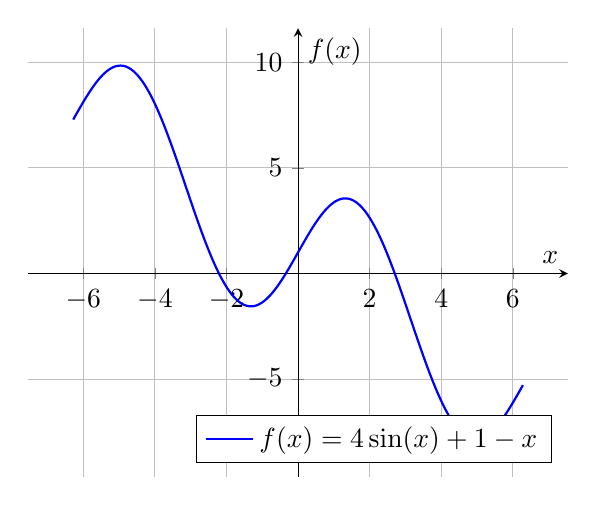
\begin{tikzpicture}
  \begin{axis}[
      axis lines=middle,
      xlabel={$x$},
      ylabel={$f(x)$},
      samples=200,
      domain=-2*pi:2*pi,
      grid=both,
      enlargelimits=true,
      legend pos=south east,
    ]
    \addplot[blue, thick] {4*sin(deg(x)) + 1 - x};
    \addlegendentry{$f(x) = 4\sin(x) + 1 - x$}
  \end{axis}
\end{tikzpicture}
\end{center}

I'm too lazy to perform the steps of the algorithm. The number of steps needed
again are given by 

\begin{equation*}
    n \geq \frac{\ln \left( \frac{4-2}{10^{-3}} \right) }{\ln 2} \approx 10.96
\end{equation*}

so taking $n = 11$ suffices.

\pagebreak 

\begin{shaded}
    \textbf{(4)} Let $a > 0$. Computing $\sqrt{a} $ is equivalent to finding the
    root of $f(x) = x^2 -  a$. 

    $(a)$ Show that Newton's sequence for this case is 

    \begin{equation*}
        x_{n+1} = \frac{1}{2}\left( x_n + \frac{a}{x_n} \right)  
    \end{equation*}

    $(b)$ Prove that f or any $x_0 > 0$, the approximations $\left\{ x_n
    \right\} $ satisfy $x_n \geq \sqrt{a} $ for $n \geq 1$. 

    $(c)$ Prove $\left\{ x_n \right\} $ is sdecreasing. 

    $(d)$ Conclude that the sequence converges to $\sqrt{a} $
\end{shaded}

$(a)$ In Newton's algorithm, 

\begin{equation*}
    x_{n+1} = x_n - \frac{f(x_n)}{f'(x_n)}
\end{equation*}

Clearly, 

\begin{equation*}
    f'(x) = \frac{d}{dx} (x^2 - a) = 2x
\end{equation*}

Therefore, 

\begin{align*}
    x_{n+1} 
    &= x_n - \frac{x_n^2 - a}{2x_n} \\ 
    &= x_n - \frac{1}{2}\left( x_n - \frac{a}{x_n} \right)  \\ 
    &= \frac{1}{2}x_n + \frac{1}{2} \frac{a}{x_n} \\ 
    &=\frac{1}{2}\left( x_n + \frac{a}{x_n} \right) \qquad \blacksquare
\end{align*}

$(b)$ Let $x_0 > 0$. Recall that, among all Pythagorean means, the arithmetic
mean is the greatest, asuming positively-valued vectors. In particular, it is
greater or equal to the geometric mean:

\begin{equation*}
    \frac{1}{N}\sum_{i=1}^n y_i \geq \sqrt[n]{\prod_{i=1}^n y_i} 
\end{equation*}

for any set of points $y_1, \ldots, y_n$ all positive. In particular, 

\begin{equation*}
    x_{n+1} = \frac{1}{2}\left( x_n + \frac{a}{x_n} \right) \geq \sqrt{x_n \frac{a}{x_n}}
    = \sqrt{a} \qquad \blacksquare
\end{equation*}

$(c)$  

\begin{align*}
&\frac{1}{2}\left( x_n + \frac{a}{x_n} \right) \leq x_n \\ 
\iff& x_n + \frac{a}{x_n} \leq 2x_n\\
\iff &\frac{a}{x_n} \leq x_n\\
\iff& a \leq x_n^2 \\ 
\iff& \sqrt{a} \leq x_n
\end{align*}

which is true due to point $(b)$.


$(d)$ Let $e_n = x_n - \sqrt{a} $. We have shown $\left\{ x_n \right\} $ to be
decreasing and bounded below by $\sqrt{a} $. Therefore, it converges to a limit
$L$ (with $L$ the infimum of $\left\{ x_n \right\} $). Then 

\begin{equation*}
    \lim_{n \to \infty} x_{n} = \frac{1}{2}\lim_{n \to \infty} \left( x_{n-1} +
    \frac{a}{x_{n-1}}\right) = \frac{1}{2}L + \frac{a}{2L}
\end{equation*}

This induces the equation 

\begin{align*}
    L = \frac{L}{2} + \frac{a}{2L} 
    &\iff \frac{L}{2} = \frac{a}{2L} \\ 
    &\iff L^2 = a\\
    &\iff L = \sqrt{a}  \qquad \blacksquare
\end{align*}

\pagebreak 

\begin{shaded}
    \textbf{(5)} Propose an iteration formula to approximate $\frac{1}{\sqrt{a}
    }$ , with $a > 0$, using Newton's method. Decide the number of iterations
    needed so that the relative error in the approximation is less than
    $10^{-4}$ when starting from $x_0 = 1$ and taking $a = 5$.
\end{shaded}

Error: $e_n = r - x_n$, quadratitc, i.e. $| r - x_{n+1}| \leq c |r - x_n|^2$.

($a$. Iteration formula) Let $a > 0$ and assume we wish to approximate $1 /
\sqrt{a} $. Let $\varphi = \frac{1}{a}$, so that $\frac{1}{\sqrt{a} } =
\sqrt{\varphi} $. We see that we can express the problem of finding the
reciprocal of a root in terms of a simple root.

We know from the previous excercise that the iteration formula for
$\sqrt{\varphi} $ is 

\begin{equation*}
    x_{n+1}=\frac{1}{2}\left( x_n + \frac{\varphi}{x_n} \right)  
\end{equation*}

Now take $x_{0} = 1$ and $a = 5$, so that
$\varphi = \frac{1}{5}$. The relative error of approximation on iteration $n$ is 

\begin{equation*}
    e_n = \frac{ \left| x_n - \frac{1}{\sqrt{5} } \right|  }{\sqrt{5} }
\end{equation*}

Brute-forcing allows us  to see that $x_0, x_1, x_2, x_3$ do not meet the criterion,
but 

\begin{equation*}
    x_4 = 0.4472137791286728 ~ (\text{ jaja } )
\end{equation*}

has $e_4 < 10^{-4}$.

\pagebreak 

\begin{shaded}
    \textbf{(6)} Propose an iteration formula for $\sqrt[3]{R} $ where $R > 0$. Plot the
    function to see where the procedure converges.
\end{shaded}
Observe that finding $\sqrt[3]{R}$ is equivalent to finding a root of $f(x) =
x^3 - R$. 

\begin{center}
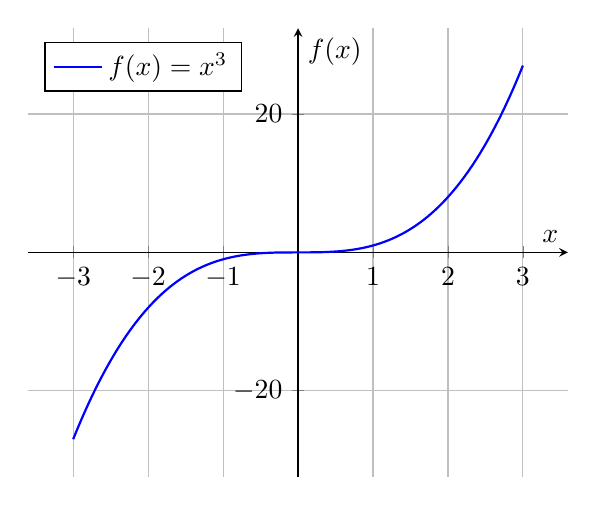
\begin{tikzpicture}
  \begin{axis}[
      axis lines=middle,
      xlabel={$x$},
      ylabel={$f(x)$},
      samples=200,
      domain=-3:3,
      grid=both,
      enlargelimits=true,
      legend pos=north west,
    ]
    \addplot[blue, thick] {x^3};
    \addlegendentry{$f(x) = x^3 $}
  \end{axis}
\end{tikzpicture}
\end{center}



But $f(x)$ is simply a vertical displacement of $x^3$, so $\frac{d}{dx} x^3 =
\frac{d}{dx} f(x)$ (which holds algebraically). In particular, the derivative
of $x^3$ approaches $0$ as $x \to 0$, meaning that Newton's method will fail to
converge for intervals of length $L$ around $0$ (with $L$ unspecified). The
graph suggests that an appropriate value for $L$ is $1$.

That said, since $\frac{d}{dx}f(x) = \frac{d}{dx} x^3$ (in other words, since
the derivative of the function is independent of $R$), and $\frac{d}{dx} x^3 =
3x^2$, we propose 

\begin{equation*}
    x_{n+1} = x_n - \frac{x_n^3}{3x_n^2} = x_n - \frac{x_n}{3} = \frac{2x_n}{3}
\end{equation*}

\pagebreak 


















\end{document}


